\clearpage
\section{Visualizing handwritten digit recognizer}
In neural networks, the first layer can be easily visualized by just simply reshaping the weights (see Figure \ref{fig:regression}), 
but extracting patterns which are recognized by further layers are not trivial. 
The main goal is to find an algorithm which with the input images can be 
enhanced to highlight the patterns that causes strongest activation in each neuron.


\begin{figure}
    \centering
    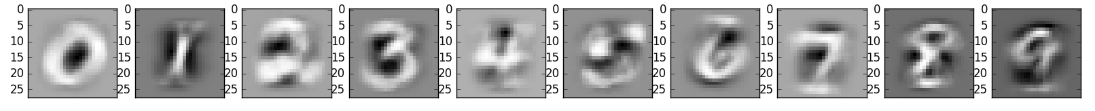
\includegraphics[width=\textwidth]{regression.png}
    \caption{Logistic regression: single layered network (without any hidden layers) trained with $L_2$ regularization can be easily visualized, because the classifier neurons are strictly connected to the input pixels. Therefore by just simply reshaping their weights to make a $28 \times 28$ image will exactly show, what each neuron is looking for on the pictures.}
    \label{fig:regression}
\end{figure}

\subsection{Training}
\label{train}
The networks were trained on the MNIST dataset \cite{mnist}, with varying the following hyperparameters:
\begin{itemize}
    \item Number of total neurons, with different distribution between layers
    \item Number of hidden layers
    \item Learning rate - constant during epochs
    \item Regularization - $L_p$
\end{itemize}

The experiments width shapes and corresponding results are shown on \emph{Figure (\ref{fig:even}, \ref{fig:dec}, \ref{fig:inc})}.
In the very beginning it turned out that networks with 3 layer are the most stable for MNIST character recognition. 
Shallow networks, with fewer layers that had theoretically larger capacity than 3 layered ones, were unable to generalize the digits.
Deeper networks, with more layers either were numerically unstable, and exhibited vanishing gradient, or overfitting occurred early in the training process.
The 3 layered networks were trained with the following constraints: Stochastic gradient descent with $mini-batch=64$, learning rate $\epsilon = 0.05$ and total number of $epochs=25$.
Despite the varying capacity, the results rather depend on the shape of the network. The best of the three networks are compared on Figure \ref{fig:comp}.


\begin{figure}
    \centering
    \includegraphics[width=0.9\textwidth]{shapeNN-even.png}
    \caption{Evenly distributed networks preserve the size of the    
    activations,    
    i.e.they map it to a space with the same dimension. 
    Despite the stable convergence during backpropagation the gradient is more likely to disappear, causing the first few layers to remain inept.}
    \label{fig:even}
\end{figure}
\begin{figure}
    \centering
    \includegraphics[width=0.9\textwidth]{shapeNN-dec.png}
    \caption{Decreasing networks tend to infer data through 
    higher levels of abstraction, from layer to layer, highest result was 
    achieved with decreasing width network}
    \label{fig:dec}
\end{figure}
\begin{figure}
    \centering
    \includegraphics[width=0.9\textwidth]{shapeNN-inc.png}
    \caption{During forward propagation the data is compressed in early layers, the later neurons rely on activation patterns of the coding layer. Networks which width of layer increase in order tends learn slower, the process is inefficient, since information is lost in the beginning.}
    \label{fig:inc}
\end{figure}

\begin{figure}
    \centering
    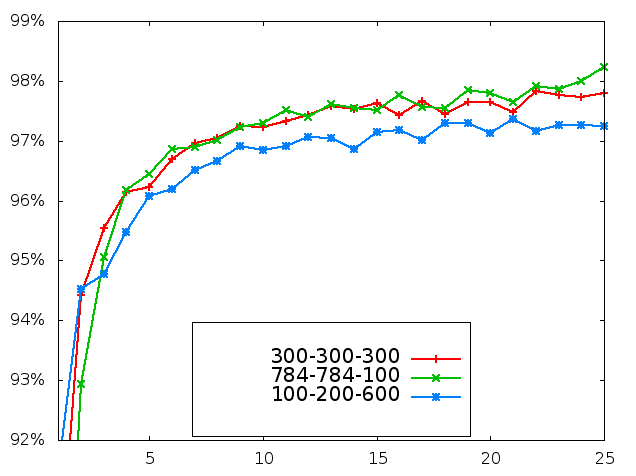
\includegraphics[width=0.9\textwidth]{comp.png}
    \caption{Comparison of the three type of distribution of neurons between layers}
    \label{fig:comp}
\end{figure}


\subsection{Candidates for enhancing}
\label{method}
The most basic method for visualizing a perceptron is cherry-picking those pictures which results in the highest output.
Formally: for a given network and set of input samples, a set of candidates can be found, which yield the highest output w.r.t. each neuron. 
For a given layer, the search can be done parallel, and for more general results, not only the best samples are taken into account, but the top $T$ inputs yielding the highest activation of all samples from the given search set, see Figure \ref{fig:ga-method1}. 
\begin{figure}
    \centering
    \includegraphics[width=0.6\textwidth]{NN1.png}
    \caption{First step of visualizing the $l^{th}$ layer: selecting each neuron's most confident choice from the image set}
    \label{fig:ga-method1}
\end{figure}
\begin{figure}
    \centeringalso 
    \includegraphics[width=0.5\textwidth]{mean-ga-comparison.png}
    \caption{On the first set of pictures the mean of the $T=100$ candidates are shown, they are the most preferred inputs of the candidate set for the last layer's neurons. On the set depicted below the enhanced images are shown}
    \label{fig:mean-ga-comp}
\end{figure}
\begin{figure}
    \centering
    \includegraphics[width=0.8\textwidth]{NN2.png}
    \caption{One iteration shown: a hidden layer's weights cannot be reshaped into images, but applying their activation gradient on the input images will emphasize, and amplify the patterns which yields the highest output w.r.t each neuron}
    \label{fig:ga-method2}
\end{figure}

\subsection{Enhancing - Gradient Ascent}

Simply mean averaging the candidates would not reveal the true signals which each neurons look for in the input space, namely the \emph{perceptive field}, see Figure \ref{fig:mean-ga-comp}.
Gradient ascent is an iterative method to determine \emph{perceptive field}, by enhancing the input to emphasize the patterns that are recognized by the neurons. 
A method which utilizes a network on top of the original to extract the recognition patterns, called DeConvnet, is described by Zeiler \emph{et al.} \cite{zeiler2014visualizing}. 
I simplified the mentioned algorithm to the following, by leaving out the sparsity encouraging regularization term - making parallel processing more efficient:
for fully connected layers the method boils down to backward propagating an \emph{arbitrary} delta vector (instead of calculating the gradient of the loss function described in \cite{zeiler2014visualizing}): 
$\delta_l = \mathbf{e}$ or $\delta_l =\mathbf{b}$
from the $l^{th}$ layer toward the input layer to get gradient of the input w.r.t the $i^{th}$ neuron's activation of the $l^{th}$ layer, and iteratively update the original sample by the gradient multiplied with \emph{modification rate}. The method is depicted on Figure \ref{fig:ga-method1} and \ref{fig:ga-method2}, 
for visual guide for understanding how the applied gradient looks like, see Figure \ref{fig:grad-sub}.

%\begin{figure}
%    \begin{subfigure}{\textwidth}
%      \centering
%      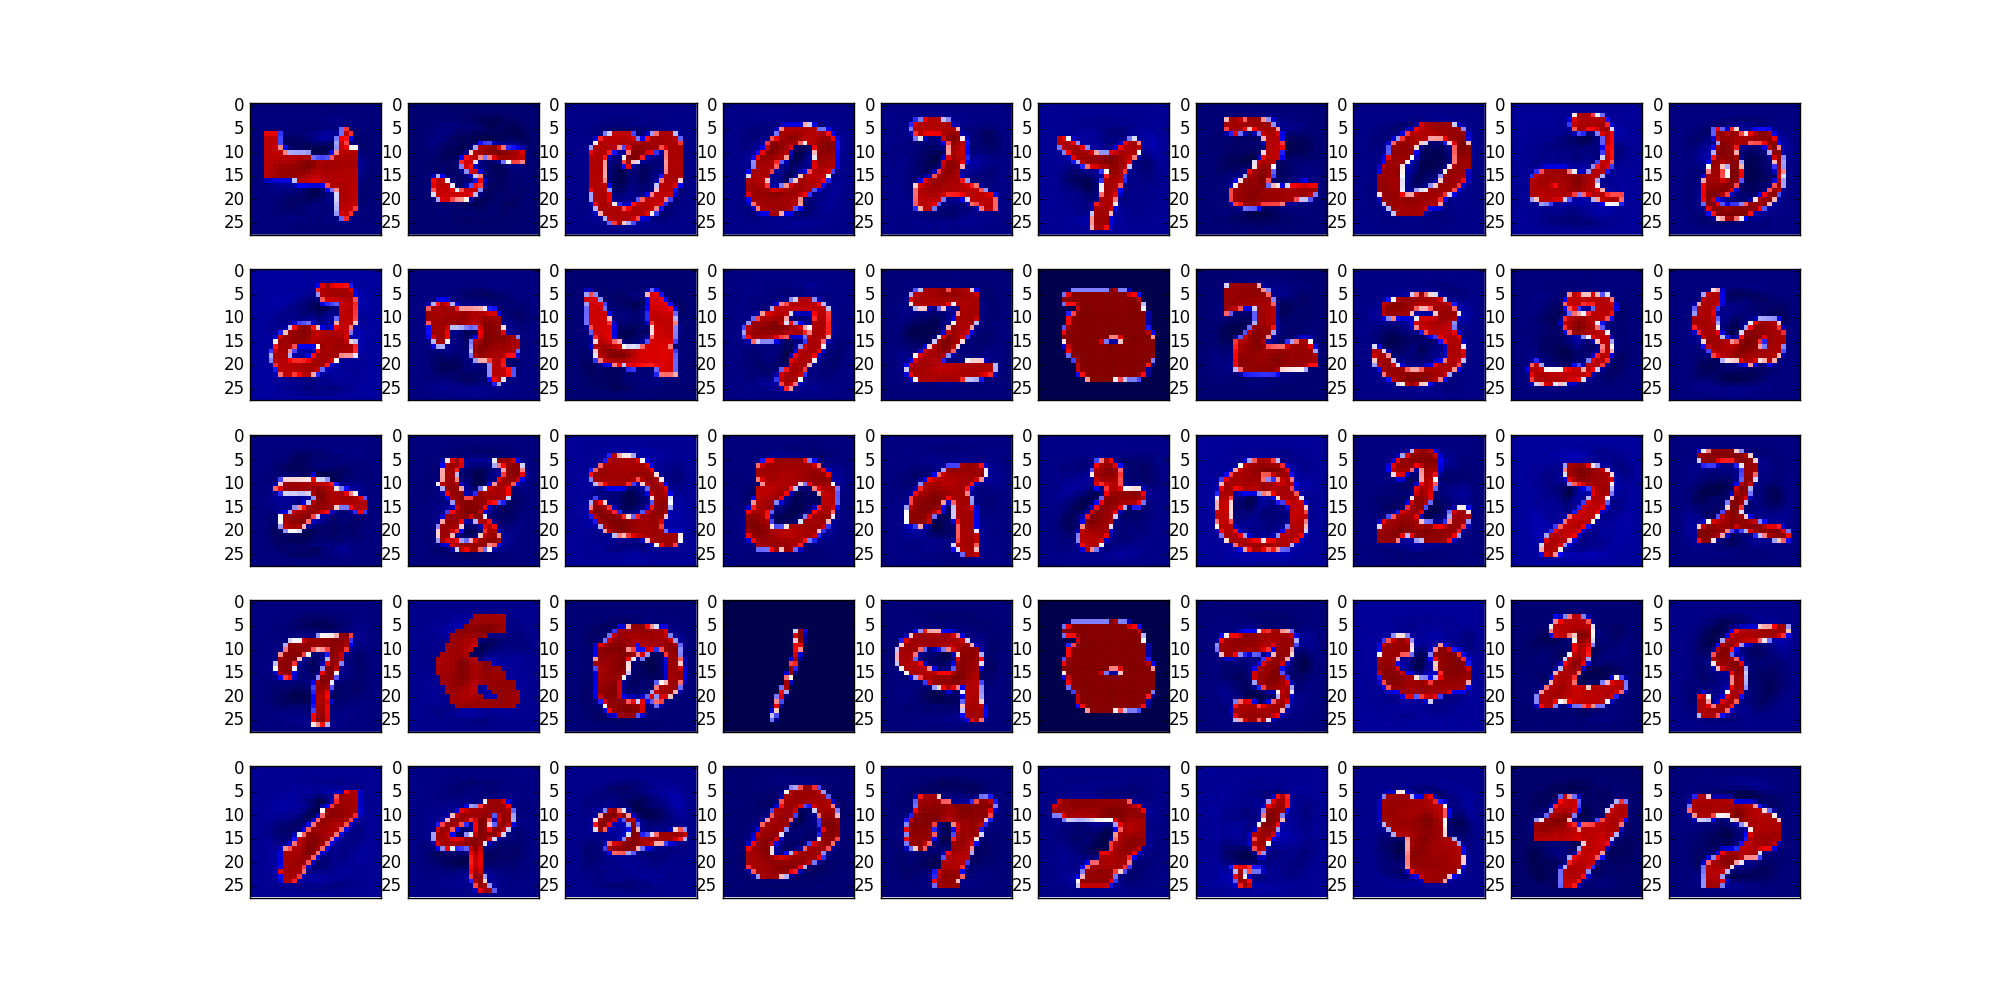
\includegraphics[width=\textwidth]{GA1.png}
%      \caption{$x+\nabla$}
%    \end{subfigure}
%%    \vfill
%    \begin{subfigure}{\textwidth}
%      \centering
%      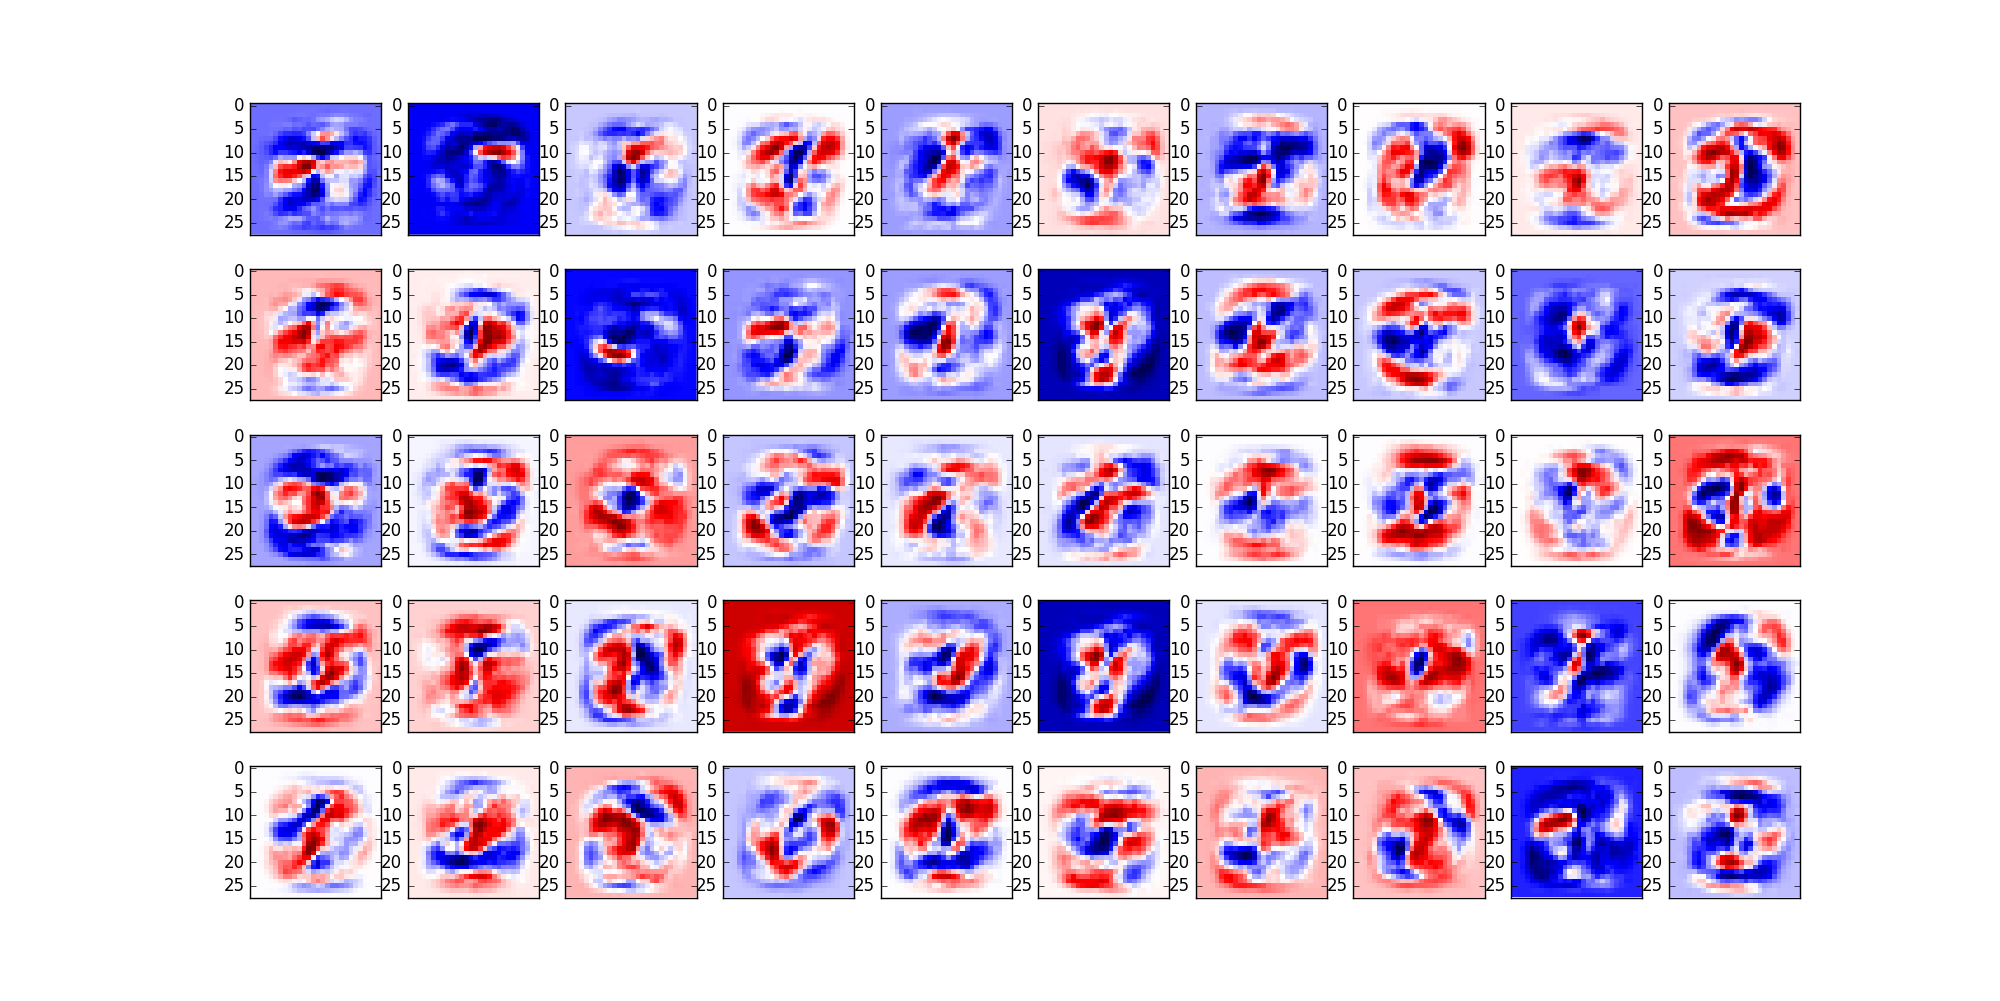
\includegraphics[width=\textwidth]{GA_gradients.png}
%      \caption{$\nabla$}
%    \end{subfigure}
%    \caption{After one iteration the enhancement is evanescent, still the gradient holds important information of the layer.
%    By looking at the gradient, we can tell which parts will be emphasized and which will be diminished during the process.
%    The depicted gradients are extracted from the randomly picked neurons from the first hidden layer of a two layered network.
%    For the smooth image result \texttt{bicubic} interpolation was used, with \texttt{seismic} color map.
%    }
%    \label{fig:grad-sub}
%\end{figure}

\begin{figure}
    \centering
    \subfloat[$x+\nabla$]{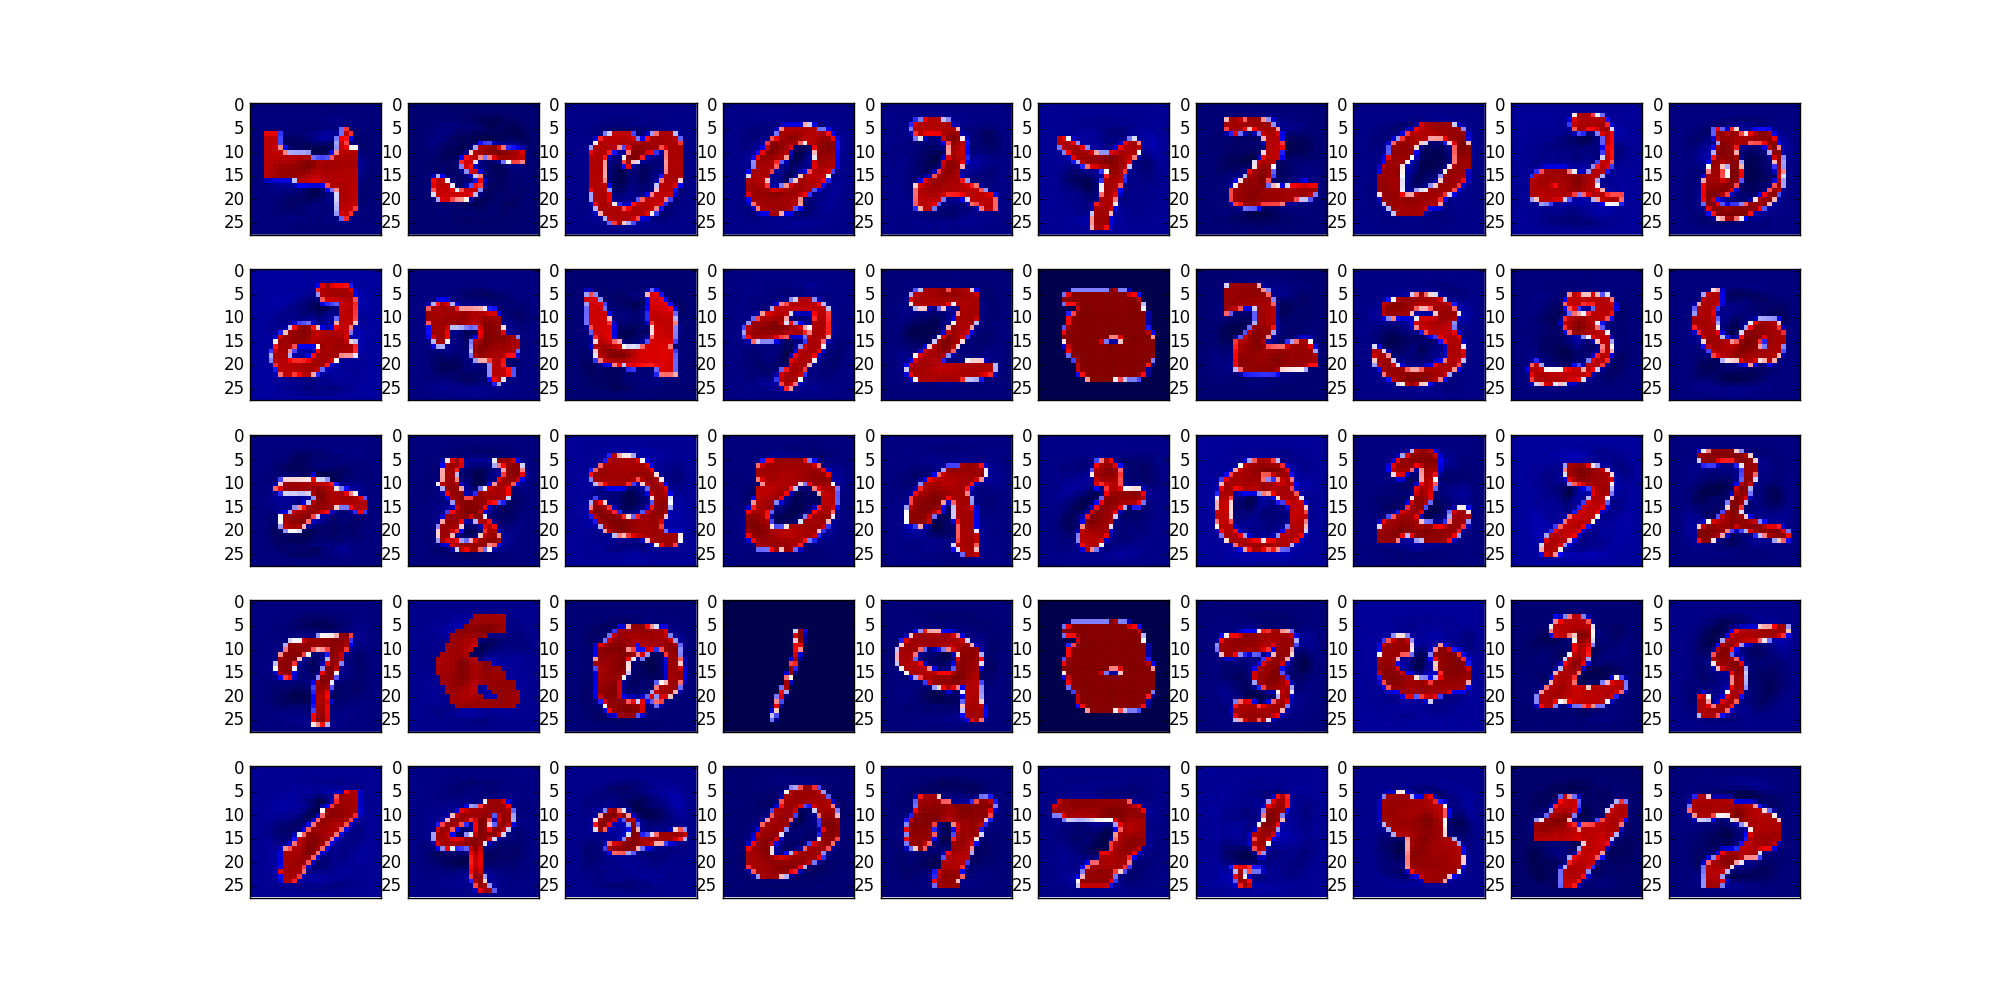
\includegraphics[width=\textwidth]{GA1.png}}\\
    \vfill
    \subfloat[$\nabla$]{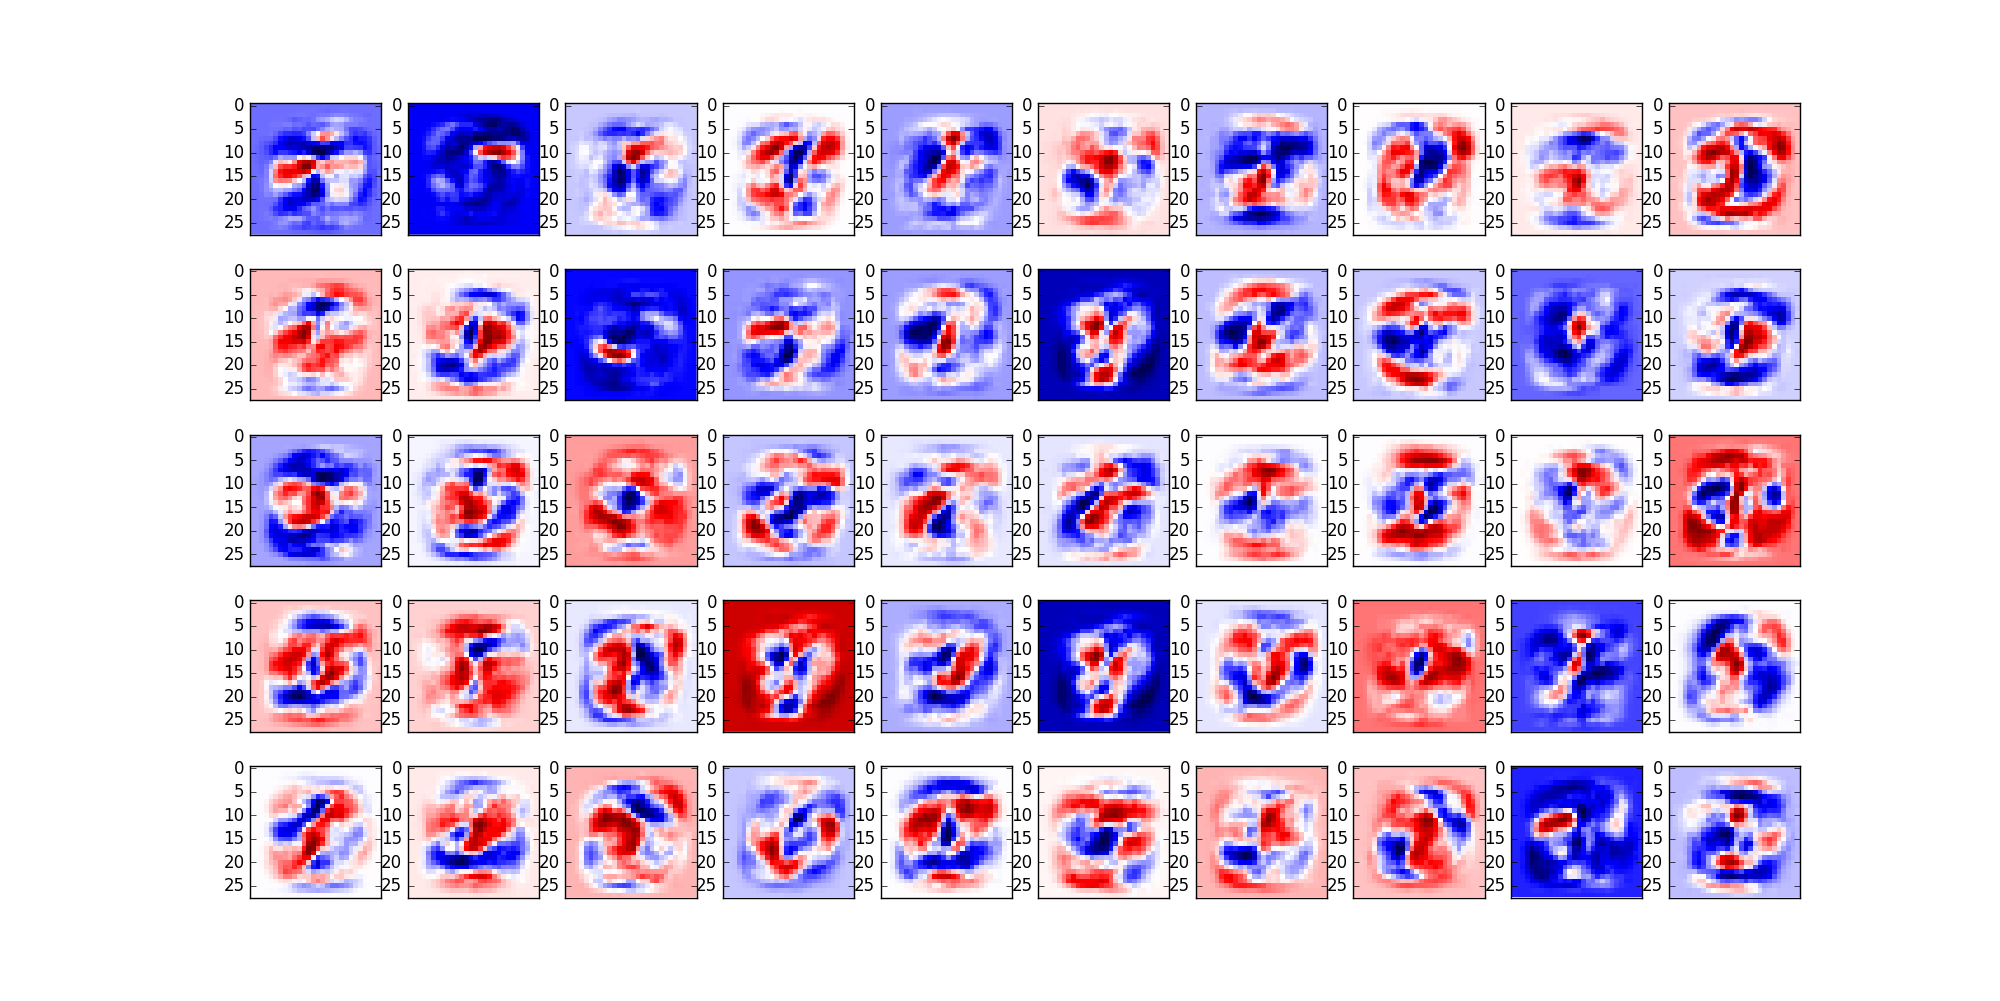
\includegraphics[width=\textwidth]{GA_gradients.png}}
    \caption{After one iteration the enhancement is evanescent, still the gradient holds important information of the layer.
    By looking at the gradient, we can tell which parts will be emphasized and which will be diminished during the process.
    The depicted gradients are extracted from the randomly picked neurons from the first hidden layer of a two layered network.
    For the smooth image result \texttt{bicubic} interpolation was used, with \texttt{seismic} color map.
    }
    \label{fig:grad-sub}
\end{figure}

In my proposed algorithm, by choosing $\mathbf{e}_{i} = [0, 0 \cdots 1 \cdots 0]^T$ the enhancement would not take other activations into account, while letting $\delta_l = \mathbf{b}_i = [-1, -1 \cdots 1 \cdots -1]^T$ would result in activation where other neurons' output would decrease over amplification. 
Both methods were tested by the following procedure: The top 1 digit was selected for each neurons in the last layer of the best performing network, totaling in 10 samples. Skipping the candidate search of the top 10 samples were enhanced by the GA algorithm, with different number of iterations and with $\mathbf{e}$ and $ \mathbf{b}$. The results are shown on Figure \ref{fig:bias-nobias}. 

\begin{figure}
    \centering
    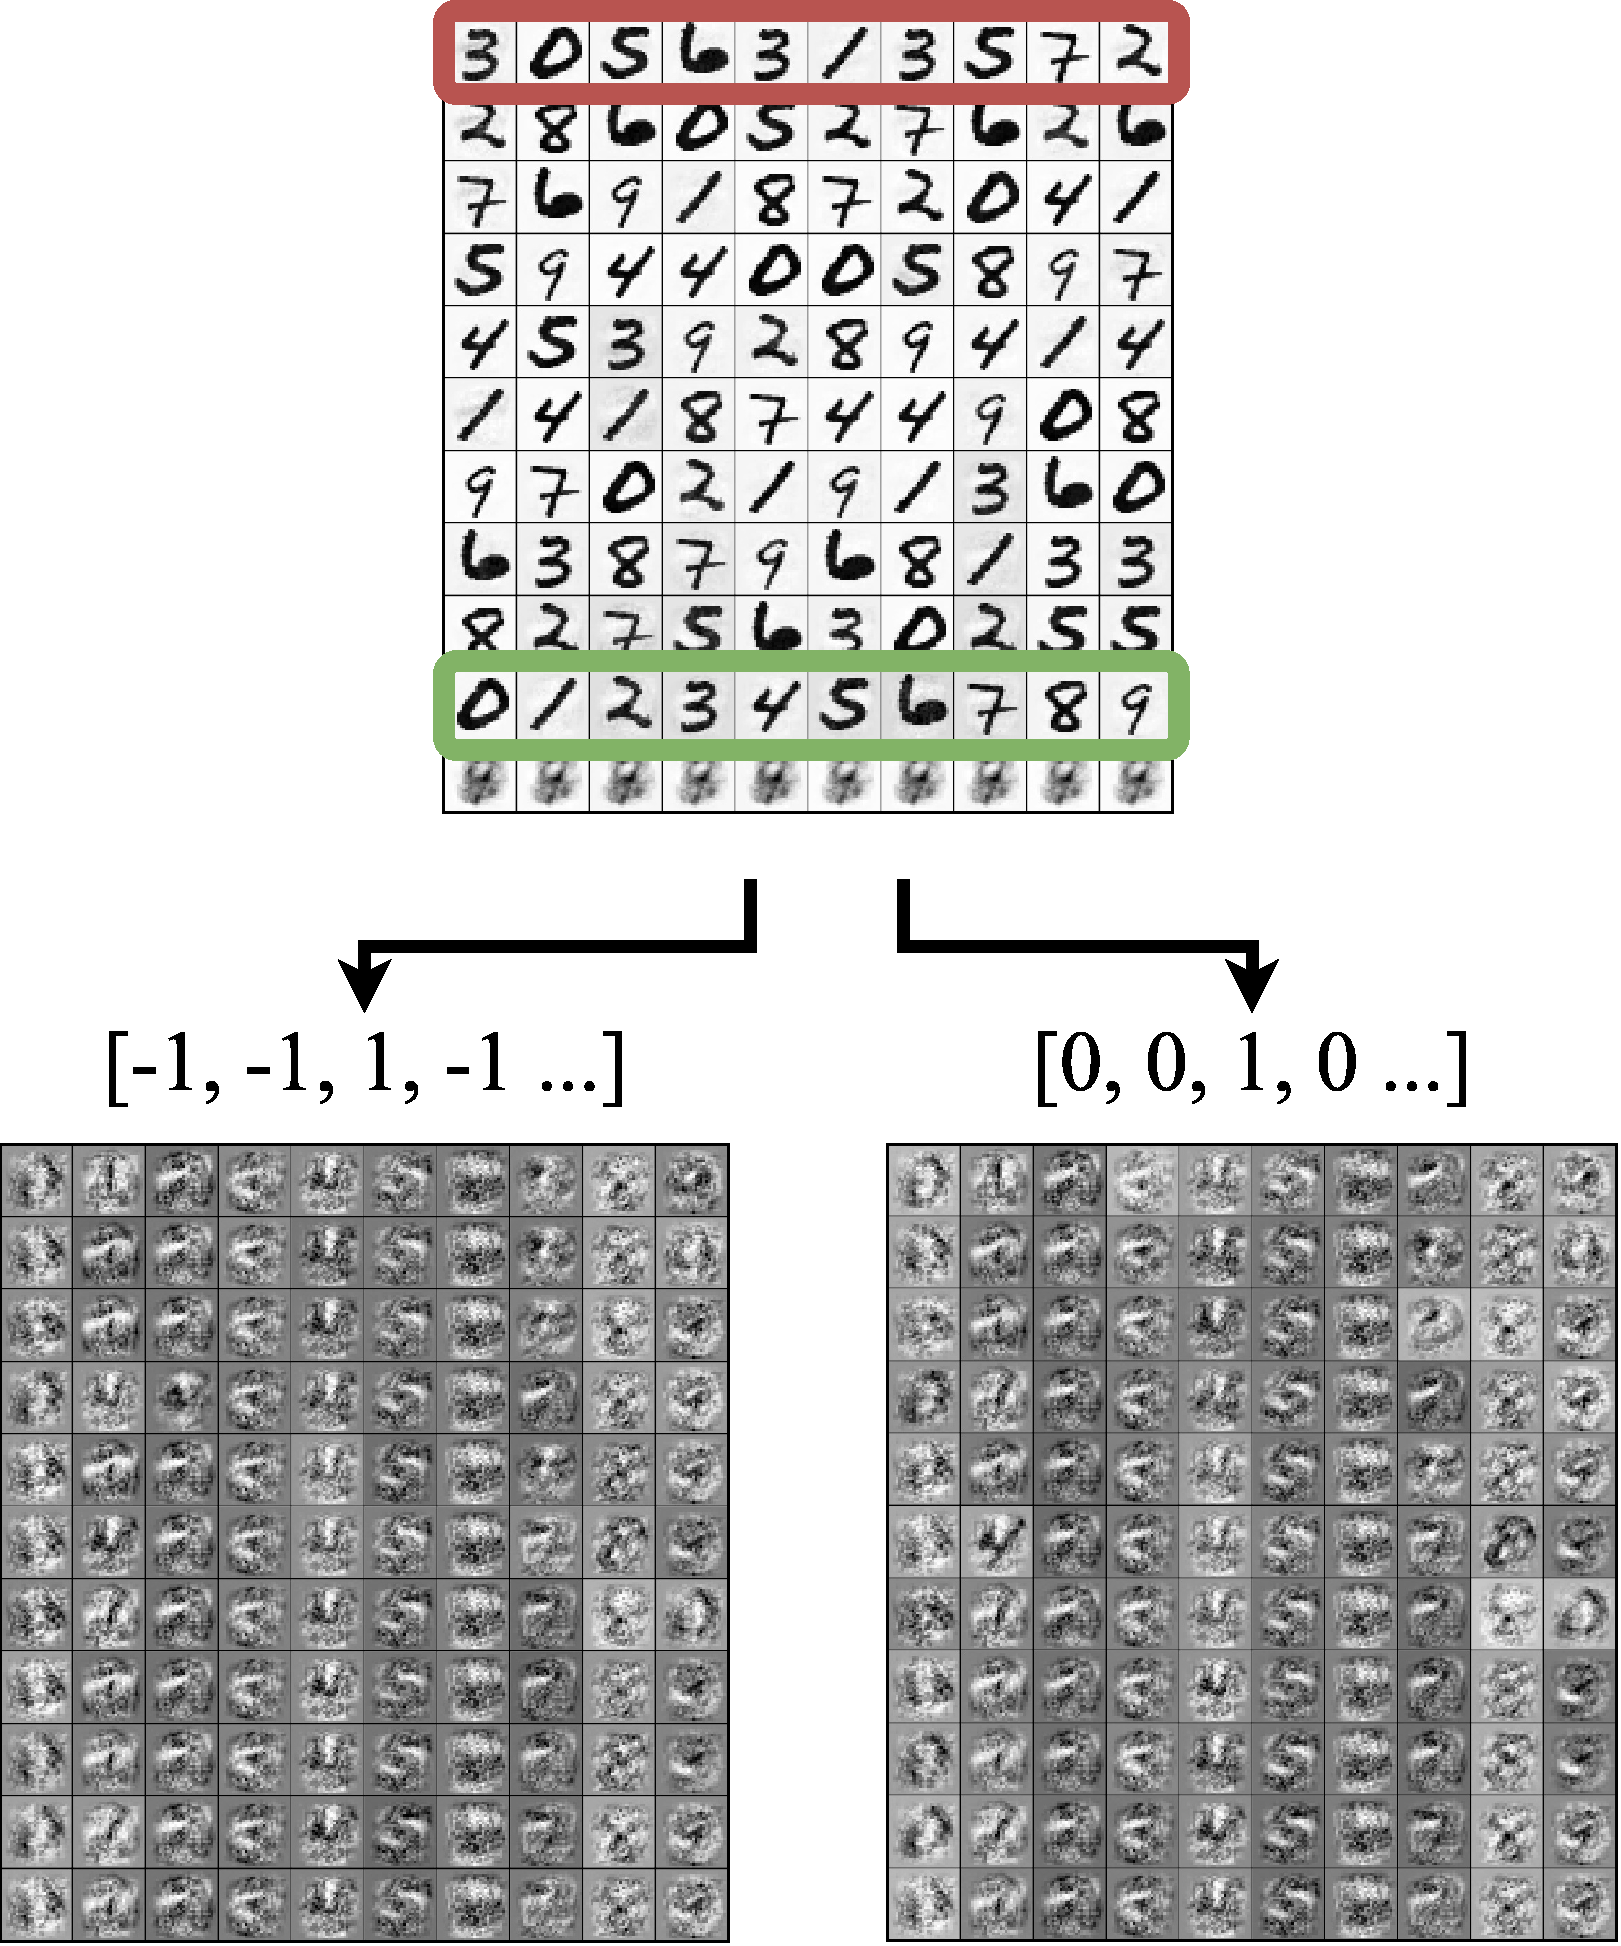
\includegraphics[width=0.9\textwidth]{bias-nobias.pdf}
    \caption{
        The different results of visualizing the last layer of a 3 layered network with 40 iterations of \emph{Gradient Ascent}. 
        Samples highlighted in green are the samples which were recognized with the highest confidence by each classifier perceptron in the last layer.
        These samples are organized in increasing order w.r.t. response of each neuron resulting in a $10 \times 10$ figure.
        \emph{Top diagram (highlighted in red)}: are the samples of the 10 candidate sample which caused the lowest activation.
        \emph{Bottom of the diagram (below the green box)}: there is a row of mean average of the samples above it, for each neuron.
        The arrows are pointing to diagrams, organized in a similar fashion, depicts samples enhanced by 
            G.A. applied with the corresponding gradient on the latent layer. 
        \emph{Left diagram}: samples enhanced by \textbf{biased} GA 40, with $rate=0.05$.
        \emph{Right diagram}: samples enhanced by \textbf{unbiased} GA 40, with $rate=0.05$.
    }
    \label{fig:bias-nobias}
\end{figure}
It is important to notice, that the algorithm initialized with different samples will introduce artifact features on the samples. 
These features will bring closer the input towards an artificial sample which will much more likely be recognized as a sample from the class of the corresponding neuron. 
The method of distortion can be exploited as well, which is called \emph{generating Adversarial} samples (detailed explanation in the end of the section).
However applying GA on the sample with the corresponding neuron (samples in the green box on Figure \ref{fig:bias-nobias}) results in much better visualization of \emph{what each node is looking for} on the input.
By qualitative analysis we concluded that biased Gradient Ascent takes less iterations to transform the sample, however applying it should be  only restricted in the classifying layer, since it is diminishing activation of neighboring neurons. 
A comparison of how the algorithms work iteration by iteration, on noise and misleading samples is shown on Figure \ref{fig:noise-GA}
    

\begin{figure}
    \centering
    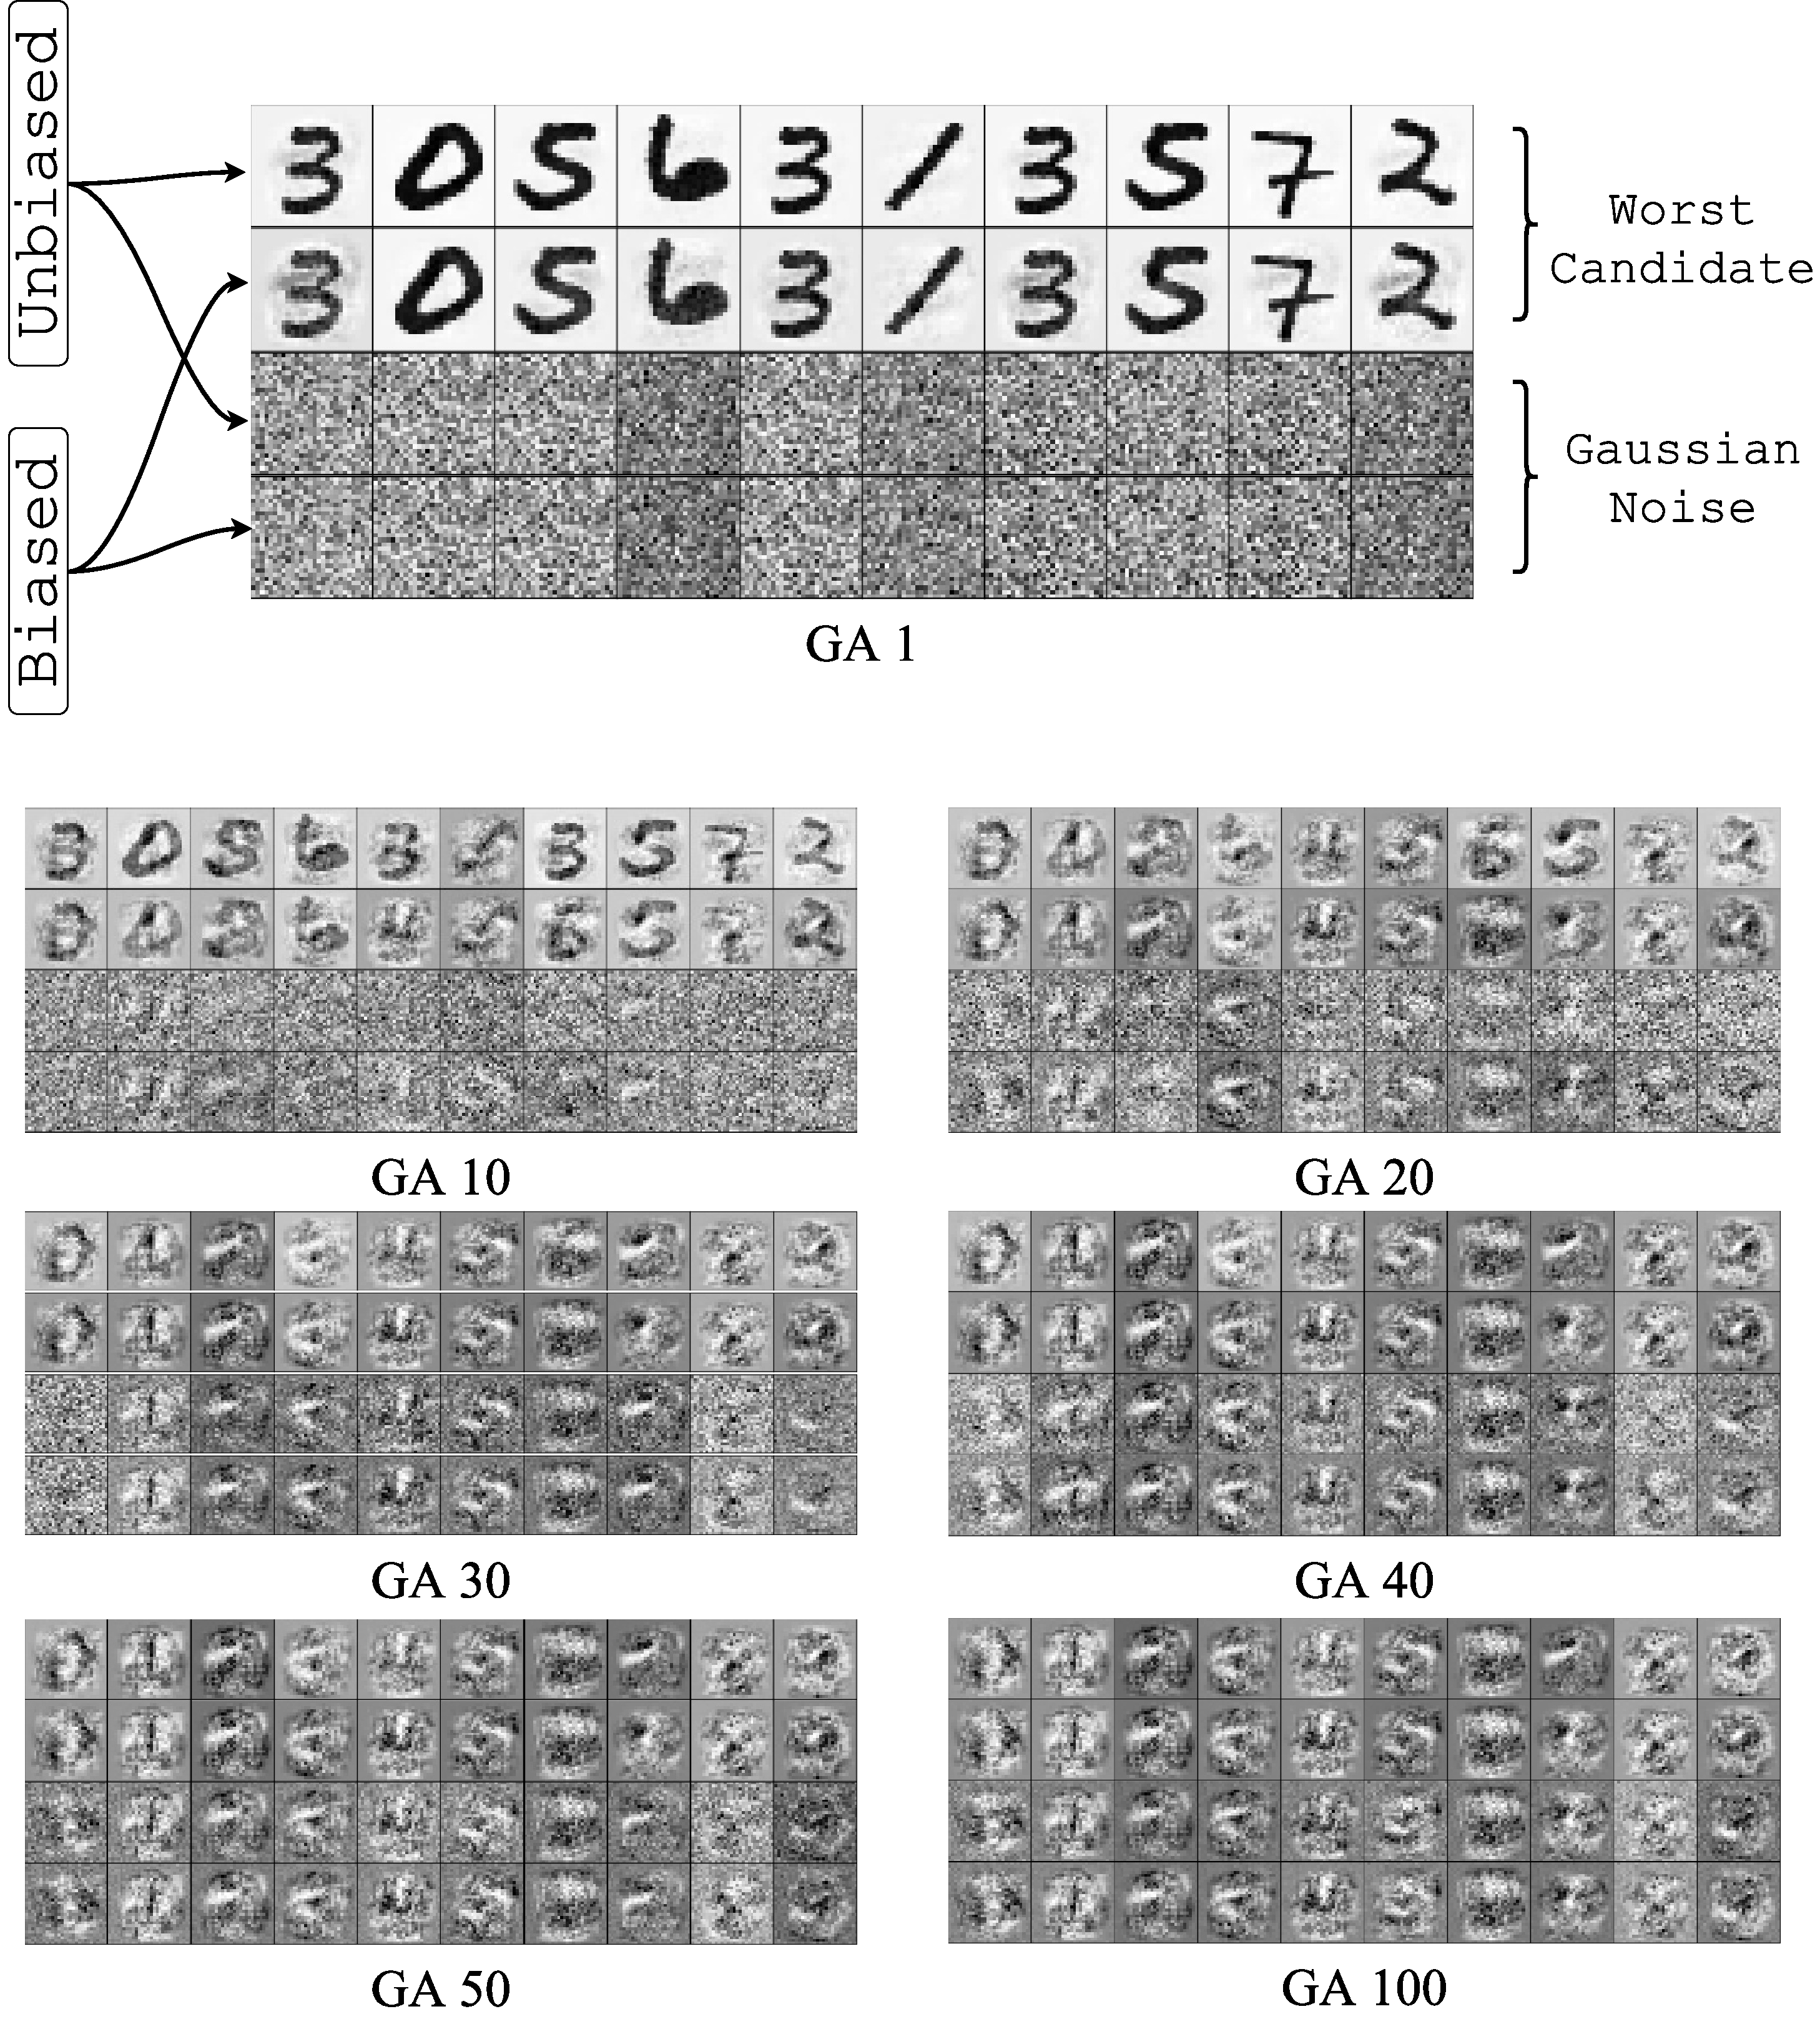
\includegraphics[width=0.9\textwidth]{noise-GA.pdf}
    \caption{Generating \emph{adversarial} samples with biased and unbiased Gradient Ascent. 
    In the first two rows, the images were enhanced by the \emph{'wrong'} gradient, making them more likely to be recognized by the corresponding classifier neuron
    $0, 1 ... 9$.
    }
    \label{fig:noise-GA}
\end{figure}

Therefore for further analysis $\mathbf{e_i} = [0, 0 \cdots 1 \cdots 0]^T$ is used.
$$x = x + \mathbf{\eta}\cdot\nabla_l^i x$$
Applying the gradient to the input $x$ is the first step of the iteration (see Figure \ref{fig:ga-method2}). Next step is forwarding the enhanced input, applying the $\delta$ on the $l^{th}$ layer and backwarding, and applying it on the input again makes a full cycle.
The hyperparameters of the method are the \emph{rate of amplification $\mathbf{\eta}$} and \emph{number of iterations $I$}

\subsection{Processing enhanced samples}
The results of amplifying the top $T$ samples for $n_l$ number of neurons in the $l^{th}$ layer are stored in a $d + 2$ dimensional matrix:
$$
    shape(\mathbf{R}) = (T, n_l, d_1, d_2, \cdots)
$$
where $d$ is the dimension of the original input.
For compact visualisation, the results are aggregated, mean averaged in the first dimension of $\mathbf{R}$ which highlights the main parts of the input, that took role in increasing the activation of the given neuron.


\subsection{Results of visualization}

A pre-trained network holds generalized information in the weights and biases, and the approach mentioned in \emph{subsection \ref{method}}, produce great amount of possible representations of the networks' inner state. In this subsection MNIST samples enhanced by parameters derived from the \emph{MLP}s trained in \emph{subsection \ref{train}} are analyzed and compared - \textit{absolutely} non exhaustively, following intuitions like:

\begin{itemize}
    \item Where, and how does abstraction occur, from combining previous layers' activation patterns
    \item How does differently distributed nodes affect the above.
    \item Do fully connected networks converge to recognizing \emph{localized} patterns, like ConvNets do
\end{itemize}

\subsection{Challenges} Because the parameter space is too wide, the main obstacle in visualization is to find out what to look for. For example visualizing the current best network that has the following dimensions: 
\begin{itemize}
    \item for each node in the network there is a $T \times 28 \times 28$ sized input set
    \item for each layer there is a given set of nodes $N = [784, 784, 100, 10]$ respectively
\end{itemize}

Totaling in $T\times(N_l)$ picture per layer, which are hard to deal with, \emph{(see Figure \ref{fig:dense})}. 
Especially when the neuron's favored patterns can be matched to different digits, 
the $T$ should be increased in order to get a more general picture when aggregating the amplified pictures.
On the other hand, the gradient ascent optimization cannot terminate on \emph{convex functions}, which is actually true for the activation of neural node's activation w.r.t to its input - meaning that the original image can be amplified as many times as possible, the output of the corresponding neuron $y_l^i$ will always increase with the number of iterations $I$. An example for applying the same method, but with 5 times the original number of iterations depicted on \emph{Figure \ref{fig:dense}} is shown on \emph{Figure \ref{fig:dense-100}}.
Therefore finding the best $I$ is also essential for extracting important information from the network.


\begin{figure}
    \centering
    \includegraphics[width=0.6\textwidth]{mean-noGA.png}
    \caption{The naive way to extract interpretable patterns is to gather those inputs which excites the most the given layer, and \textbf{mean average} it. The case depicted on the figure, is that the ideal input is not trivial as the listed candidates shows, especially in the first layers. By aggregating}
    \label{fig:mean}
\end{figure}


\begin{figure}
    \centering
    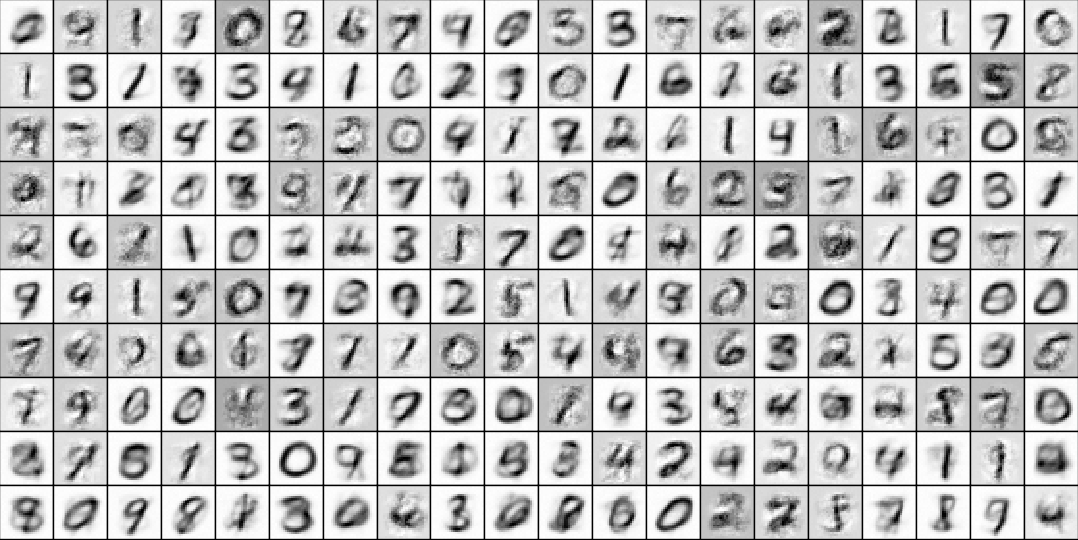
\includegraphics[width=0.9\textwidth]{200-dense-GA20.png}
    \caption{Iteratively enhanced pictures of the first hidden layer of a \textbf{[300-300-300]} network (first 200 are shown in \emph{row-major order}). The main question is, which of them holds important features, or needs further analysis.}
    \label{fig:dense}
\end{figure}


\begin{figure}
    \centering
    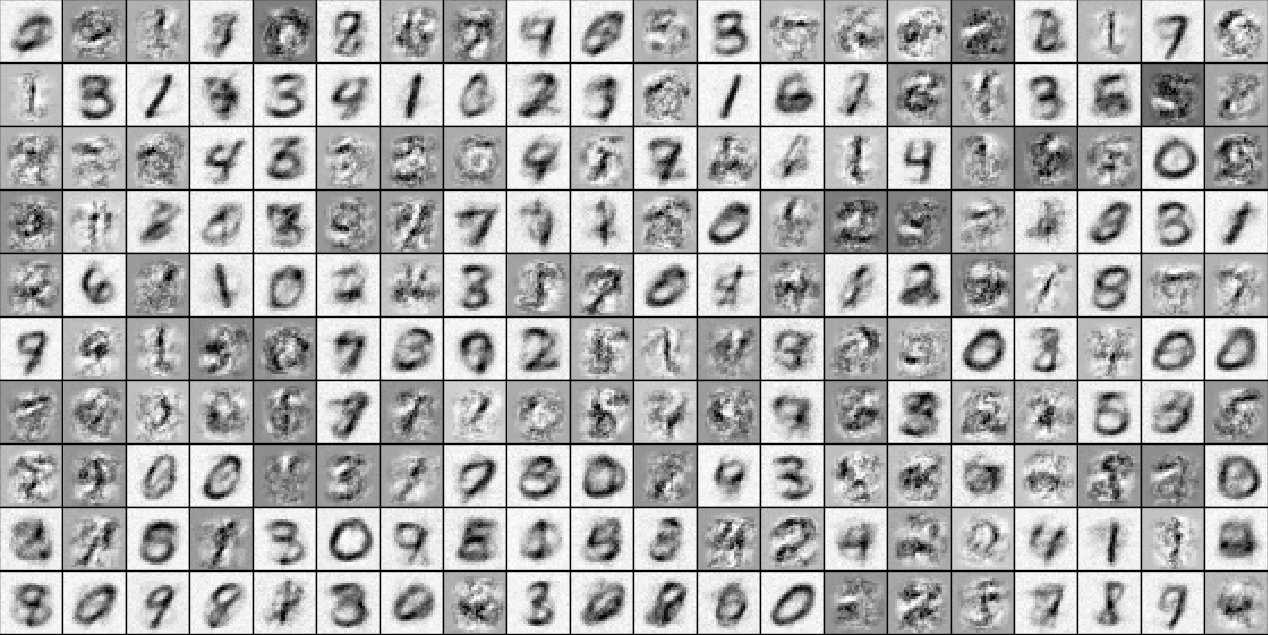
\includegraphics[width=0.9\textwidth]{200-dense-GA100.png}
    \caption{After increasing $T$, compared to fig. \ref{fig:dense} some of the amplified pictures gets noisy, which is not a problem in the first case. It is a trend in the early layers, to only focus on small, localized type of features, that yields different candidates, which makes the mean of the outcome noisy overall. Especially this is one important feature of \emph{MLPs} that initialized with random weights they converge towards recognizing localized features.}
    \label{fig:dense-100}
\end{figure}


\emph{\textbf{Note}: Deviating, or averaging the input samples is an important step to strengthen the features which the given node truly recognize, and drop out those which it does not (see Figure \ref{fig:mean}). For the rest of the case studies mean averaging is used for aggregation}

\textbf{Remainder}: For the following examples, a small subset of samples are shown, which were selected for the most revealing clues. Still, they may not represent all features of the network.


\subsection{Analyzing the best performing network}
The best result belongs to a network with hidden layer width: 784-784-100. 
The layers were visualized with the following parameters:
$T=100$
$\eta=0.1$
$I=10, 50$
and the training set was used for choosing candidates.

The suggestion while looking for evidences is that the reason behind the good performance of the network is relying on different levels of abstraction.
I visualized all three layers in order to get a better grasp what happens inside of a network, which can recognize digits with $98\%$ success.
For conviction, that we cannot simply read the values out from neither the activation, or the weights from the hidden layers see Figure \ref{fig:act-weight}.

\begin{figure}
    \centering
    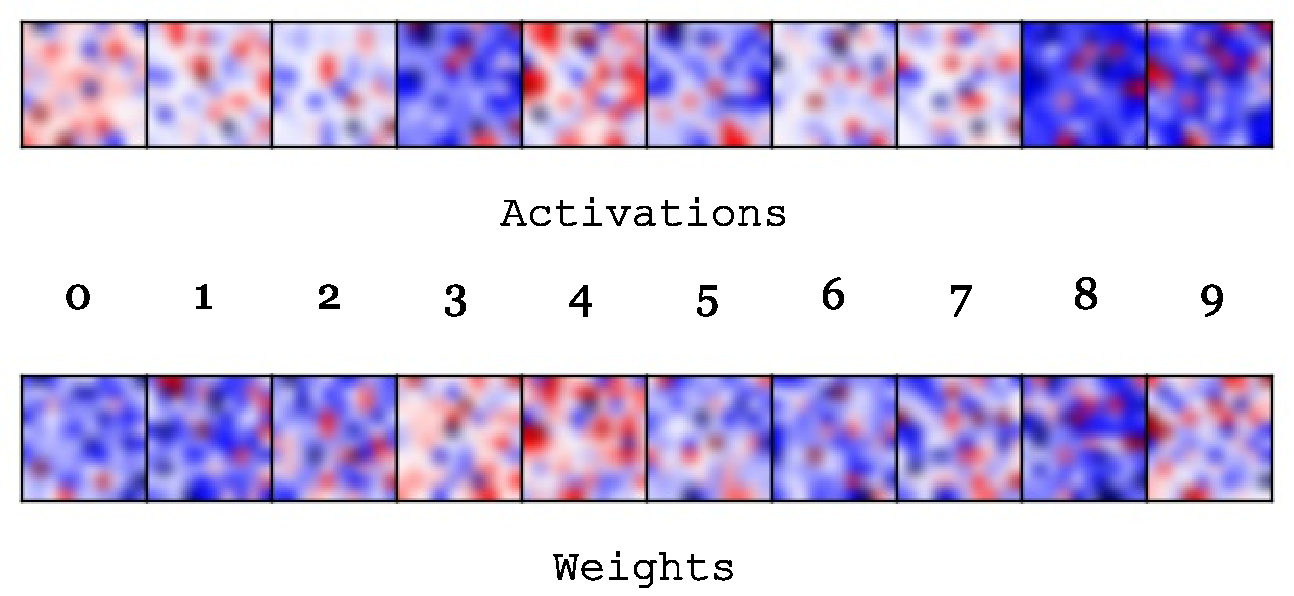
\includegraphics[width=0.9\textwidth]{act-weight.pdf}
    \caption{\emph{On top}: Every sample translates to some response signal (like the depicted maps) before reaching the final classifier layer. 
    Though we cannot understand it, for the network the activation patterns holds all information about the corresponding input.
    \emph{On bottom}: Each map is processed by the weights of the last layer, which is also essential for the network, but does not exhibit any intuitive feature.
    Think about the analogy: we cannot simply define what happens inside by just looking at brains of creatures. 
    Even if we had a high resolution microscope, revealing the fine structure of the nervous tissue would not suddenly illuminate everything.
    }
    \label{fig:act-weight}
\end{figure}